\chapter{Geometry}

\section{Q1}

  \begin{figure}[H]
    \centering
    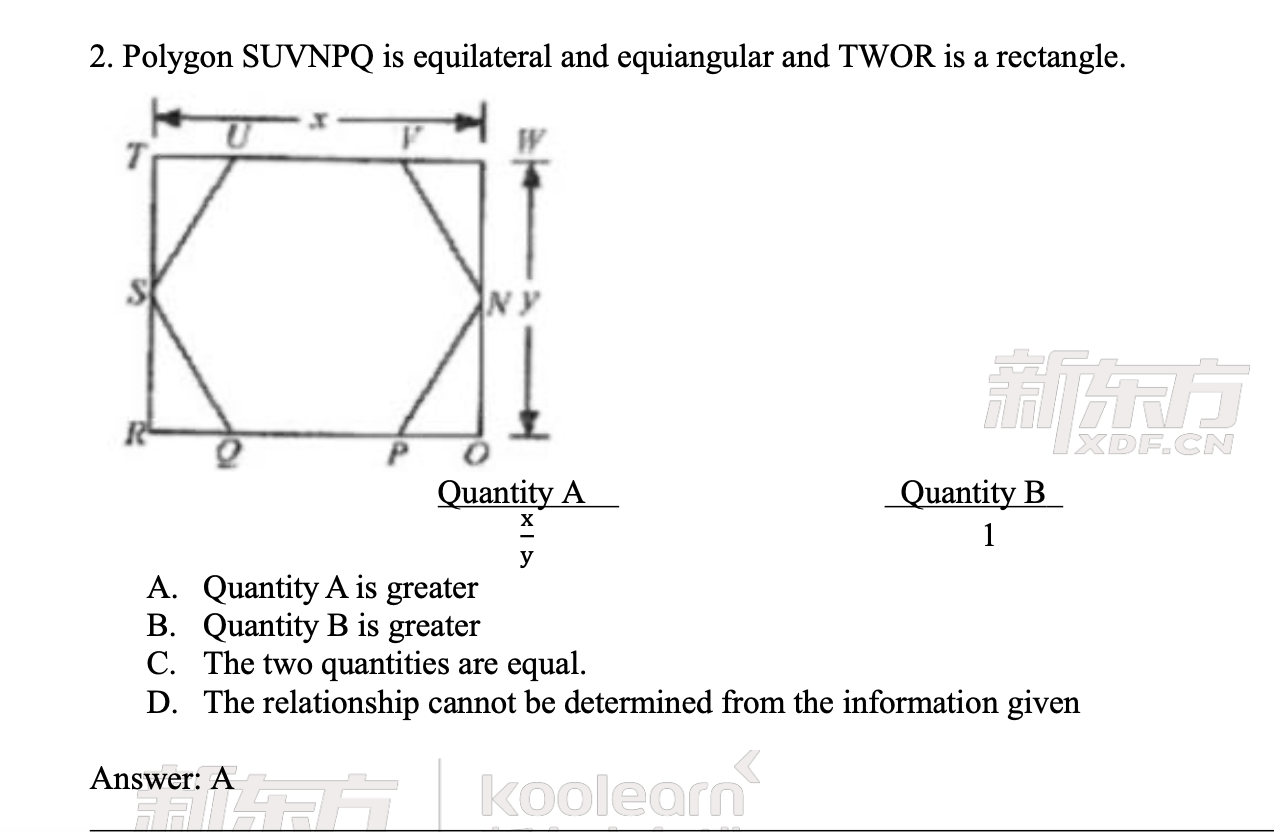
\includegraphics[width=0.7\columnwidth]{images/areas/geometry/q1}
  \end{figure}

\section{Q2}

  If $ x > 0 $, and two sides of a certain triangle have lengths $ 2 x + 1 $
  and $ 3 x + 4 $ respectively, which of the following could be the length of
  the third side of the triangle?

  \begin{enumerate}
    \item $ 4x + 5 $
    \item $ x + 2 $
    \item $ 6x + 1 $
    \item $ 5x + 6 $
    \item $ 2x + 17 $
  \end{enumerate}

  \subsection{解析}

    本题考查三角形两边之和大于第三边, 注意\textbf{could be}

    \textbf{答案}: A, C, E

\section{Q3}

  \begin{figure}[H]
    \centering
    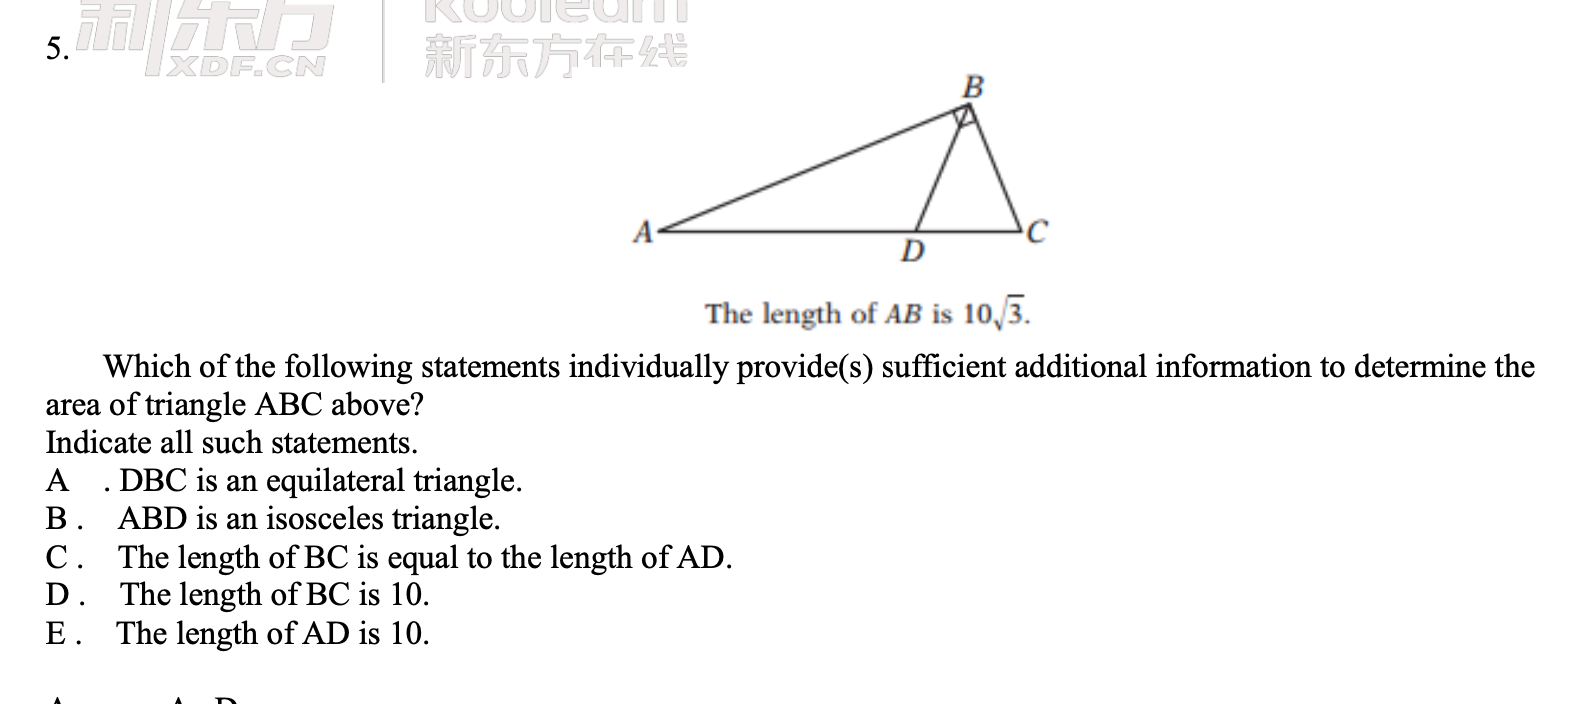
\includegraphics[width=0.7\columnwidth]{images/areas/geometry/q3}
  \end{figure}

  \subsection{解析}

    主要目标位找到$ BC $

    \begin{itemize}
      \item \textbf{A}: 等边三角形, 30度所对直角边为斜边的一半,
      $ BC = DC = \frac{AC}{2} $, 解方程可得 $ BC $
    \end{itemize}

    \textbf{答案 A, C}
